%!TEX program = pdflatex
%!TEX encoding = UTF-8 Unicode

\documentclass[11pt, a4paper]{article}

% ============================================================================
% PACKAGES
% ============================================================================

\usepackage[T1]{fontenc}
\usepackage[margin=1in]{geometry}
\usepackage{amsmath}
\usepackage{amssymb}
\usepackage{graphicx}
\usepackage{xcolor}
\usepackage{listings}
\usepackage{fancyhdr}
\usepackage{setspace}
\usepackage{enumitem}
\usepackage{booktabs}
\usepackage{tikz}
\usepackage[most]{tcolorbox}
\usepackage{helvet}
\renewcommand{\familydefault}{\sfdefault}
\usepackage{titlesec}

% ============================================================================
% CONFIGURATION
% ============================================================================

% Colors
\definecolor{codebackground}{RGB}{246, 248, 250}
\definecolor{codebordercolor}{RGB}{87, 178, 255}
\definecolor{codekeyword}{RGB}{207, 34, 46}
\definecolor{codestring}{RGB}{3, 47, 98}
\definecolor{codecomment}{RGB}{87, 96, 106}
\definecolor{codetextcolor}{RGB}{31, 35, 40}

% Clean modern code listing style (GitHub-inspired)
\newtcblisting{codebox}{
    enhanced,
    listing only,
    colback=codebackground,
    colframe=codebordercolor,
    coltext=codetextcolor,
    boxrule=0.8pt,
    arc=3pt,
    boxsep=0pt,
    left=2.5mm,
    right=2.5mm,
    top=1.5mm,
    bottom=1.5mm,
    listing options={
        language=bash,
        basicstyle=\ttfamily\small\color{codetextcolor},
        keywordstyle=\color{codekeyword}\bfseries,
        stringstyle=\color{codestring},
        commentstyle=\color{codecomment}\itshape,
        breaklines=true,
        breakatwhitespace=true,
        tabsize=4,
        showspaces=false,
        showstringspaces=false,
        columns=fixed,
        basewidth=0.5em,
        keepspaces=true,
        escapeinside={(*@}{@*)},
        literate=
            {\#}{{\#}}1
            {\_}{{{\textunderscore}}}1
    }
}

% Inline code style (matches codebox)
\newcommand{\inlinecode}[1]{%
    \raisebox{-0.2ex}{%
    \tcbox[
        enhanced,
        nobeforeafter,
        colback=codebackground,
        colframe=codebordercolor,
        coltext=codetextcolor,
        boxrule=0.5pt,
        arc=2pt,
        boxsep=0pt,
        left=0.8mm,
        right=0.8mm,
        top=0.3mm,
        bottom=0.3mm,
        fontupper=\ttfamily\small\color{codetextcolor}
    ]{#1}%
    }%
}

% Notebox style (clean modern boxes)
\tcbset {
  base/.style={
    arc=0mm, 
    bottomtitle=0.5mm,
    boxrule=0mm,
    colbacktitle=black!10!white, 
    coltitle=black, 
    fonttitle=\bfseries, 
    left=2.5mm,
    leftrule=1mm,
    right=3.5mm,
    title={#1},
    toptitle=0.75mm, 
  }
}

\definecolor{brandblue}{rgb}{0.34, 0.7, 1}
\newtcolorbox{mainbox}[1]{
  colframe=brandblue, 
  base={#1}
}

\newtcolorbox{subbox}[1]{
  colframe=black!30!white,
  base={#1}
}

% Hyperref package and styling (must be loaded near the end)
\usepackage{hyperref}
\hypersetup{
    colorlinks=true,
    linkcolor=blue,
    filecolor=blue,
    urlcolor=blue,
    citecolor=blue,
    pdftitle={Agentic Project Management - Research Study Participation Guide (Copilot)},
    pdfauthor={Konstantinos Chaidemenos}
}

% Header and footer
\pagestyle{fancy}
\fancyhf{}
\rhead{\small Participation Guide (Copilot)}
\lhead{\small Agentic Project Management Research Study}
\cfoot{\thepage}
\renewcommand{\headrulewidth}{0.5pt}

% Line spacing
\onehalfspacing

% Section formatting
\titleformat{\section}[hang]{\Large\bfseries}{\thesection.}{0.5em}{}
\titleformat{\subsection}[hang]{\large\bfseries}{\thesubsection.}{0.5em}{}

% ============================================================================
% DOCUMENT
% ============================================================================

\begin{document}

% Title Page
\begin{titlepage}
    \centering
    \vspace*{3cm}

    {\fontsize{26}{30}\selectfont\bfseries Agentic Project Management}\par
    \vspace{0.2cm}
    {\fontsize{16}{20}\selectfont \mdseries An enhancement of the emerging paradigm of\\Spec-Driven Development}\par
    \vspace{2cm}
    {\fontsize{18}{22}\selectfont \underline{Research Study Participation Guide}}\par
    \vspace{0.5cm}
    {\fontsize{16}{20}\selectfont \mdseries \underline{Sub-Study B: GitHub Copilot}}\par
    
    \begin{center}
        
\includegraphics[width=0.15\textwidth]{assets/copilot/githubcopilot.png}
    \end{center}
    \vspace{1cm}
    
    {\normalsize \textbf{Conducted by:}\\Konstantinos Chaidemenos - CobuterMan}\par
    \vspace{0.5cm}
    {\normalsize \textbf{Institution:}\\National and Kapodistrian University of Athens}\par
    \vspace{0.2cm}
    \begin{center}
        
\includegraphics[width=0.3\textwidth]{assets/common/uoa-logo.jpeg}
    \end{center}
    \vfill
    
    {\small November 2025}\par
    
\end{titlepage}

% ============================================================================

\section{Welcome \& Introduction}

Thank you for participating in this research study. Your participation is essential for evaluating how effectively modern AI-powered development tools support Spec-Driven Development (SDD) workflows.\newline\newline
The goal of this study is to compare how different AI-assisted frameworks perform on a practical, well-defined coding task. Please be assured that \textbf{you are not being tested}; the AI tools are. All data, including incomplete or non-functional code, is valuable to this research.

\subsection*{Data Privacy \& Anonymity}
All data that you will submit will be handled with strict confidentiality. Your name or any personal identifiers will not be linked to the data. The research artifacts you will provide will be used exclusively for this academic research and will be anonymized in any resulting publications. By proceeding, you consent to the anonymous collection and use of this data as described.

% ============================================================================

\section{Study Overview}

\subsection{Your Task}

Your task is to research an existing legacy PHP codebase and implement a new feature in an existing Python codebase based on your findings. You will receive a detailed \textbf{Product Requirements Document (PRD)} as the sole source of truth for the specification, guiding both you and the AI tools.

\subsection{Your Tools}

You will complete this task \textbf{twice}, each time using a different AI-coding framework (e.g., APM, Spec-kit, Copilot's Plan agent). Sessions will be \textbf{time-boxed and isolated on separate branches}. Between sessions, you will submit your code changes, chat logs, and a brief survey.

\begin{mainbox}{Learning Effects Note}
We acknowledge that performing the task twice may introduce learning effects. To mitigate this, some participants will begin with Tool A, others with Tool B. This counterbalancing aims to ensure fair assessments across the study.
\end{mainbox}

\subsection{Your Time}

Each session is strictly time-boxed to \textbf{three (3) hours}. It is important that you stop at the 3-hour mark, regardless of whether you are finished. Committing unfinished work is a perfectly valid and expected outcome.

\newpage

\subsection{Your Environment}
\label{sec:your-environment}
To ensure the two sessions are completed in a controlled environment, set up your environment according to the following specifications:
\begin{itemize}
    \item \textbf{Operating System:} POSIX-compliant systems such as Linux (e.g., Ubuntu 22.04+) or macOS (latest versions). For Windows, we recommend using Windows Subsystem for Linux (WSL) with a recent Ubuntu distribution.
    \item \textbf{APM v0.5.0+:} Make sure you have the latest version of APM installed for one of your sessions.
    \item \textbf{Workspace:} A dedicated directory with the following repositories cloned:
    \begin{itemize}
        \item \href{https://github.com/sdi2200262/eclass-mcp-server}{\texttt{eclass-mcp-server}} (the main codebase where you will implement the new feature).\\
        Install dependencies using: \inlinecode{cd eclass-mcp-server \&\& uv sync --dev --all-extras}
        \item \href{https://github.com/gunet/openeclass}{\texttt{openeclass}} (the legacy PHP codebase where you will conduct research)
    \end{itemize}
    \item \textbf{Python Version: 3.10+}
    \item \textbf{C Development Libraries:} Ensure the following C development libraries are installed for the task:
    \begin{itemize}
        \item \textbf{Ubuntu/Debian:} \inlinecode{sudo apt-get install libcurl4-openssl-dev libxml2-dev}
        \item \textbf{macOS (Homebrew):} \inlinecode{brew install curl libxml2}
    \end{itemize}
    \item \href{https://code.visualstudio.com/}{\textbf{IDE: Visual Studio Code}} of at least version \href{https://code.visualstudio.com/updates/v1_106}{1.106}
    \item \href{https://github.com/features/copilot}{\textbf{AI Tool: GitHub Copilot}}
    \begin{mainbox}{Important Copilot Access Note}
    This study requires access to GitHub Copilot's premium features. Note that \textbf{verified students are eligible for the GitHub Education Pack}, which provides free access to GitHub Copilot Pro. You can sign up for the GitHub Education Pack for free at:
    \href{https://education.github.com/pack}{\texttt{https://education.github.com/pack}}
    \newline\newline
    Please ensure you have access to GitHub Copilot's premium features in VS Code before beginning the session.
    \end{mainbox}
\end{itemize}

\subsection{What You Will Deliver}
At the end of each session, you will submit:
\begin{itemize}
    \item A \textbf{code patch file} containing all changes made during the session. For example, a patch file \inlinecode{tool\_a\_solution.patch} for Tool A and \inlinecode{tool\_b\_solution.patch} for Tool B.
    See \hyperref[sec:creating-patch]{Section~\ref*{sec:creating-patch}} for instructions on creating the patch file.
    \item The complete \textbf{AI interaction logs}, including exported chat conversations and Copilot request usage from your sessions. For example \inlinecode{tool\_a\_logs.zip} and \inlinecode{tool\_b\_logs.zip}.
    See \hyperref[sec:exporting-logs]{Section~\ref*{sec:exporting-logs}} for exporting AI interaction logs from VS Code (Copilot).
    \item A brief \textbf{post-session survey} about your experience using each AI-coding framework.
    See Sections \hyperref[sec:tool-a-survey]{\ref*{sec:tool-a-survey}} and \hyperref[sec:session-2-tool-b]{\ref*{sec:session-2-tool-b}} for links to the surveys.
\end{itemize}

\newpage
% ============================================================================

\section{AI Tools: Setup \& Instructions}
\label{sec:ai-tools}

Before starting your sessions, familiarize yourself with your assigned tools. Below are setup instructions and usage guidelines for each tool.

\subsection{APM in VS Code (Copilot)}

\subsubsection*{Description:}

\href{https://github.com/sdi2200262/agentic-project-management/}{\textbf{Agentic Project Management (APM)}} is designed to enhance your development process by decomposing specifications into actionable tasks and coordinating their execution across multiple AI agents; aiming to improve efficiency and context management.

\subsubsection*{Setup Instructions:}

\begin{itemize}
    \item Ensure you have \inlinecode{npm} installed on your system.
    \item Install the \inlinecode{agentic-pm} package globally using the following command:
    \begin{codebox}
npm install -g agentic-pm
    \end{codebox}
    \item Once installed, use the \inlinecode{apm init} command within your working directory's root (alongside the other codebases) and select \inlinecode{GitHub Copilot}.
\end{itemize}

\subsubsection*{Video Tutorial \& Familiarization:}

To get acquainted with APM watch this \href{https://www.youtube.com/watch?v=dQw4w9WgXcQ}{tutorial} and/or read the \href{https://github.com/sdi2200262/agentic-project-management/tree/main/docs}{official documentation} before starting your timed session.

\subsection{Spec-kit in VS Code (Copilot)}

\subsubsection*{Description:}

\href{https://github.com/github/spec-kit}{\textbf{Spec-kit}} is another AI-powered development framework designed to enhance the specification and planning stages of software development, ensuring a spec-first approach throughout the implementation process.

\subsubsection*{Setup Instructions:}

\begin{itemize}
    \item Ensure \inlinecode{uv} has been installed and set up on your system.
    \item Install the \inlinecode{specify-cli} using their official recommended installation command:
    \begin{codebox}
uv tool install specify-cli --from git+https://github.com/github/spec-kit.git
    \end{codebox}
    \item Once installed, use the \inlinecode{specify init <your-project-name>} command within your working directory's root (alongside the other codebases) and select \inlinecode{GitHub Copilot}.
\end{itemize}

\newpage
% ============================================================================

\subsubsection*{Video Tutorial \& Familiarization:}

To get acquainted with Spec-kit watch this \href{https://www.youtube.com/watch?v=a9eR1xsfvHg}{tutorial} and/or read the \href{https://github.github.com/spec-kit/}{official documentation} before starting your timed session.

\subsection{Plan agent in Copilot}

\subsubsection*{Description:}

Copilot's \textbf{Plan agent} implements Spec-Driven Development principles by emphasizing a "first-plan-then-execute" workflow. The agent is designed to research a task, break it down into manageable steps, ask clarifying questions, and present a full implementation plan \textbf{before} any code is written.

\subsubsection*{Setup Instructions:}

No additional setup is required beyond having VS Code with GitHub Copilot installed.
To enable the Plan agent, select it from the agent picker of Copilot's Chat panel:

\begin{center}
    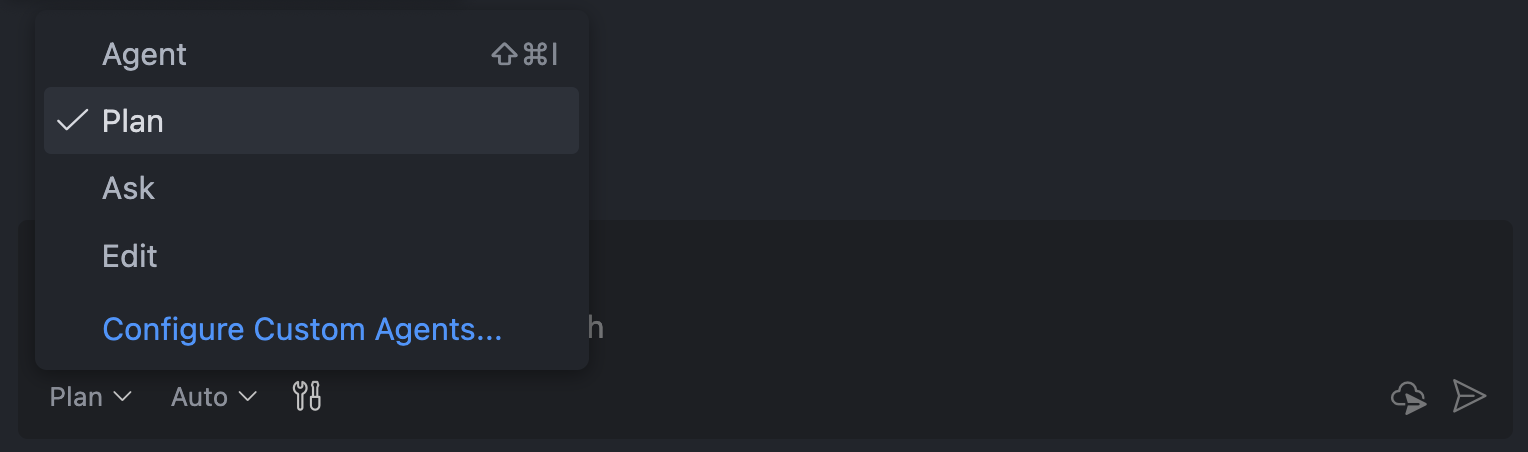
\includegraphics[width=1\textwidth]{assets/copilot/copilot-plan-agent.png}
\end{center}

\subsubsection*{Video Tutorial \& Familiarization:}

The Plan agent is integrated directly into Copilot. For a brief overview, see Copilot's official documentation on the \href{https://code.visualstudio.com/docs/copilot/chat/chat-planning}{Plan agent}.

\vspace{1.2cm}
\hrule height 0.3pt
\vspace{0.7cm}

\begin{mainbox}{Important Familiarization Note}
Before starting your timed session, it is \textbf{crucial} to familiarize yourself with the features and workflows of your assigned tool by watching the provided tutorials and reviewing the relevant documentation. You are encouraged to practice using the tool on small, unrelated tasks to build confidence. However, \textbf{please avoid using the actual task or codebase during practice to minimize learning effects.}\newline\newline
\textbf{This preparation will help you use the tool effectively during the task.} In the post-session survey, you will be asked about your experience and familiarity with the tool.
\end{mainbox}


\newpage
% ============================================================================

\section{Session Workflow (Step-by-Step)}

This section explains the session workflow in which you are to attempt to complete your task. Please follow these steps in order.

\subsection{Ensure Environment is Set Up}

Following \hyperref[sec:your-environment]{Section~\ref*{sec:your-environment}}, ensure you have installed VS Code with GitHub Copilot and that you have correctly set up your environment with all dependencies installed and the required repositories. You may include the \inlinecode{Specification.md} and the \inlinecode{Default\_Prompt.md} files alongside this guide in your workspace for your convenience.\newline\newline
Opening VS Code in your designated workspace directory would look like this:
\begin{center}
    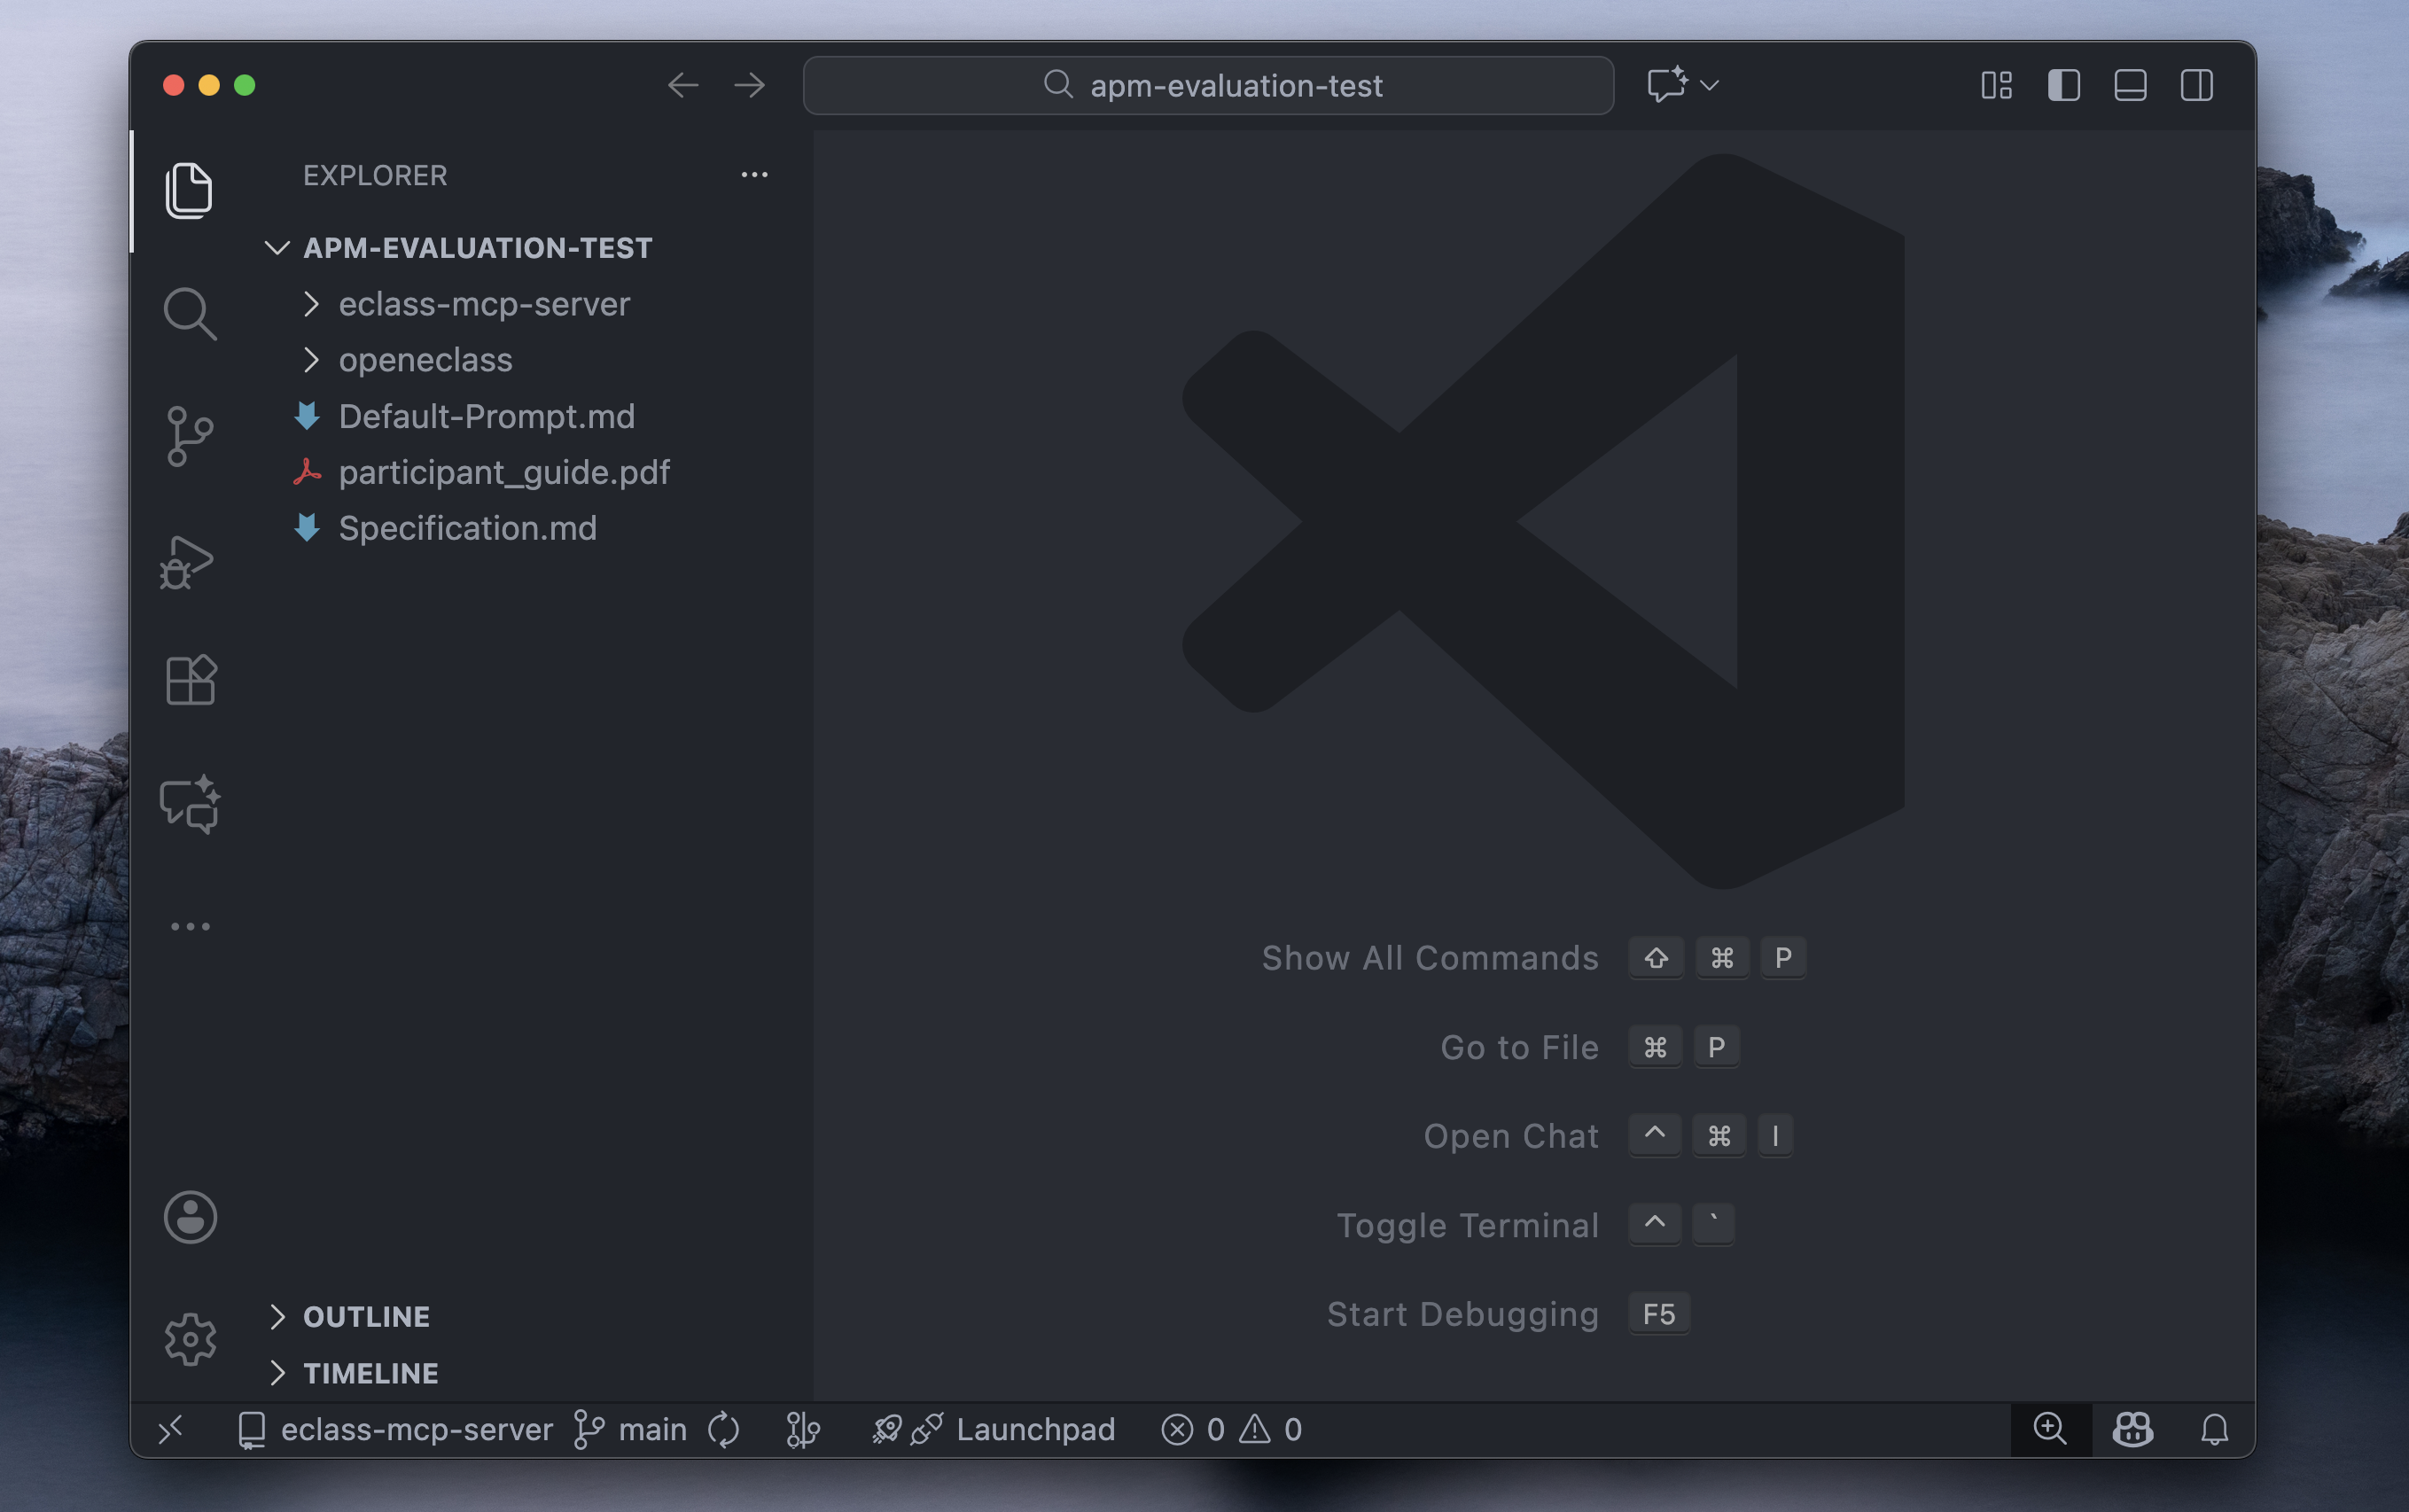
\includegraphics[width=1\textwidth]{assets/copilot/copilot-setup.png}
\end{center}
\noindent Verify that all the base dependencies are installed by running:
\begin{codebox}
/PATH/TO/YOUR/PYTHON3 --version   # Check Python version
uv --version                      # Check UV version  
npm --version                     # Check NPM version (for APM)

# Check Python codebase dependencies (silent success, errors shown)
cd eclass-mcp-server
/PATH/TO/YOUR/PYTHON3 -c "import mcp"
/PATH/TO/YOUR/PYTHON3 -c "import requests"
/PATH/TO/YOUR/PYTHON3 -c "import bs4"
/PATH/TO/YOUR/PYTHON3 -c "import dotenv"
\end{codebox}

\subsection{Session 1: Tool A}


\subsubsection*{Initialize Git and Create Branch:}
    
    Ensure you're starting from a clean state and create an isolated branch:
    \begin{codebox}
cd eclass-mcp-server                # go to implementation codebase root
git checkout main                   # switch to main branch
git checkout -b tool-a-attempt      # create new branch for Tool A patch
    \end{codebox}

\subsubsection*{Before you start working:}
    
    \begin{itemize}
        \item Launch your first assigned AI tool (Tool A) following its setup instructions in \hyperref[sec:ai-tools]{Section~\ref*{sec:ai-tools}}.
        \item \textbf{Thoroughly read the} \inlinecode{Specification.md} (the PRD) provided alongside this guide.
        \item Use the \textbf{Default Prompt} provided alongside this guide to initiate your conversation with your AI tool.
        \item Take a screenshot of the Copilot \textbf{Premium Requests usage bar} from your GitHub Copilot Settings page; this will serve as the \textbf{start-of-session} usage baseline.
        \item Use \textbf{only} your assigned Tool A for AI assistance during this session.
        \item Start the timer and get to work!
        
        \begin{mainbox}{Important Copilot Workflow Note}
            Due to Copilot's request-based billing, participants should follow a \textbf{Hybrid Model strategy} when using these tools. This is to conserve your request quota.
            \begin{itemize}
                \item \textbf{APM sessions:}
                \begin{itemize}
                    \item \textbf{Setup Phase:} Use \textbf{Claude Sonnet 4} for the initial \textbf{Setup Agent} session.
                    \item \textbf{Task Loop Phase:} Keep using \textbf{Claude Sonnet 4} for the \textbf{Manager Agent} and switch to whichever non-premium model you prefer for the \textbf{Implementation Agents} throughout the task execution. Non-premium models are the ones with a 0x multiplier in the model picker.
                \end{itemize}
                \vspace{0.5em}
                \item \textbf{Plan Agent and Spec-kit sessions:} use \textbf{Claude Sonnet 4} for planning and non-premium for execution.
            \end{itemize}
        \end{mainbox}
    \end{itemize}
        
\subsubsection*{Work Until Completion or Time Limit:}
    
    \begin{itemize}
        \item Iterate on the task for \textbf{up to 3 hours}.
        \item \textbf{Stop at the 3-hour mark}, even if you haven't completed the task.
        \item Alternatively, stop when you have fully completed the task \textbf{(if before 3 hours)}.
    \end{itemize}

\subsubsection*{Create Code Patch:}
\label{sec:creating-patch}

    After the 3 hour mark or upon task completion, generate your solution patch file for this session:
    \begin{codebox}
git add . && git commit -m "Tool A solution"            # commit all changes
git diff main tool-a-attempt > tool_a_solution.patch    # create patch file
    \end{codebox}
    \begin{mainbox}{Git Note}
Feel free to use Git for version control during your session. However, ensure that you \textbf{do not modify the main branch directly}. All code changes related to your task should be committed to your isolated branch (\inlinecode{tool-a-attempt} for Tool A and \inlinecode{tool-b-attempt} for Tool B) before concluding the session.
    \end{mainbox}

\subsubsection*{Export AI Interaction Logs:}

Follow the specific instructions in \hyperref[sec:exporting-logs]{Section~\ref*{sec:exporting-logs}} to export chat conversations and retrieve request statistics. Save these as \inlinecode{tool\_a\_logs.zip}.

\subsubsection*{Clean Up and Ensure Isolation:}

    Return to main branch and remove the solution branch:
    \begin{codebox}
git checkout main
git branch -D tool-a-attempt
    \end{codebox}
        \begin{mainbox}{Important Branch Isolation Note}
At this step, you will remove all changes made during the Tool A session from your local repository. Ensure that you have successfully created the patch file and exported all logs before proceeding, as these changes will no longer be recoverable.
        \end{mainbox}

\subsubsection*{Complete Tool A Survey:}
\label{sec:tool-a-survey}

Fill out the brief \href{https://forms.gle/dPJY5vYg6XwU4T5b8}{Tool A post-session survey}.


\subsubsection*{Session 1 Checklist:}
\label{sec:session-1-checklist}
Before moving to Session 2, ensure you have completed the following:
\begin{itemize}
    \item Created the patch file \inlinecode{tool\_a\_solution.patch} and deleted the \inlinecode{tool-a-attempt} branch.
    \item Collected AI interaction logs and packaged them as \inlinecode{tool\_a\_logs.zip}:
    \begin{itemize}
        \item Exported all chat conversations and packaged them as \inlinecode{tool\_a\_chat\_conversations.zip}.
        \item Captured Copilot request usage screenshots as \inlinecode{tool\_a\_copilot\_requests\_start/end.png}.
    \end{itemize}
    \item Completed the \href{https://forms.gle/dPJY5vYg6XwU4T5b8}{Tool A post-session survey}.
\end{itemize}

\newpage
% ============================================================================

\subsection{Session 2: Tool B}
\label{sec:session-2-tool-b}

Follow the same workflow as Session 1, but with the following adjustments:

\begin{itemize}
    \item Create a branch named \inlinecode{tool-b-attempt} from the clean \inlinecode{main} branch.
    \item Use \textbf{Tool B} following its setup instructions in \hyperref[sec:ai-tools]{Section~\ref*{sec:ai-tools}}.
    \item After the 3 hour mark or upon task completion, generate the patch file as \inlinecode{tool\_b\_solution.patch}:
    \begin{codebox}
git diff main tool-b-attempt > tool_b_solution.patch
    \end{codebox}
    \item Export logs as \inlinecode{tool\_b\_logs.zip} following the same procedure as Tool A.
    \item Complete the \href{https://forms.gle/dPJY5vYg6XwU4T5b8}{Tool B post-session survey}.
    
    \begin{mainbox}{Important Session 2 Note}
        You may start Session 2 immediately after Session 1 or take a break. Ensure you are ready to approach Session 2 from scratch, maintaining a fresh perspective and minimizing any influence from Session 1.\newline\newline
        To accurately collect all data from Session 2, please \textbf{make absolutely sure you capture both start and end Copilot usage screenshots for this session and that you have all the artifacts from \hyperref[sec:session-1-checklist]{Section~\ref*{sec:session-1-checklist}}}.
    \end{mainbox}
\end{itemize}

\subsubsection*{Session 2 Checklist:}
\label{sec:session-2-checklist}
Before concluding your work, ensure you have completed the following:
\begin{itemize}
    \item Created the patch file \inlinecode{tool\_b\_solution.patch} and deleted the \inlinecode{tool-b-attempt} branch.
    \item Collected AI interaction logs and packaged them as \inlinecode{tool\_b\_logs.zip}:
    \begin{itemize}
        \item Exported all chat conversations and packaged them as \inlinecode{tool\_b\_chat\_conversations\_json.zip}.
        \item Captured Copilot request usage screenshots as \inlinecode{tool\_b\_copilot\_requests\_start.png} and \inlinecode{tool\_b\_copilot\_requests\_end.png}.
    \end{itemize}
    \item Completed the \href{https://forms.gle/dPJY5vYg6XwU4T5b8}{Tool B post-session survey}.
\end{itemize}

\newpage
% ============================================================================

\section{Exporting AI Interaction Logs from VS Code (Copilot)}
\label{sec:exporting-logs}

To export your AI interaction logs (chat conversations and AI request statistics) from Copilot, follow these steps for both sessions.

\subsection{Export Chat Conversations}
When using Tools A or B, you may open multiple chat conversations (e.g., at least three with APM: Setup, Manager, and Implementation Agents; one or two with Spec-kit or Plan agent). \textbf{Retain all chat conversations for our analysis. Do not delete any during your sessions}. To export chats, follow these steps:
\begin{itemize}
    \item For each chat conversation opened during your session, \textbf{navigate to that specific chat} in the VS Code sidebar so it is your \textbf{active, visible chat tab}.
    \item Open the Command Palette (\inlinecode{Cmd+Shift+P} on macOS or \inlinecode{Ctrl+Shift+P} on Windows/Linux).
    \item Type and run the \textbf{"Chat: Export Chat..."} command.
    \begin{center}
        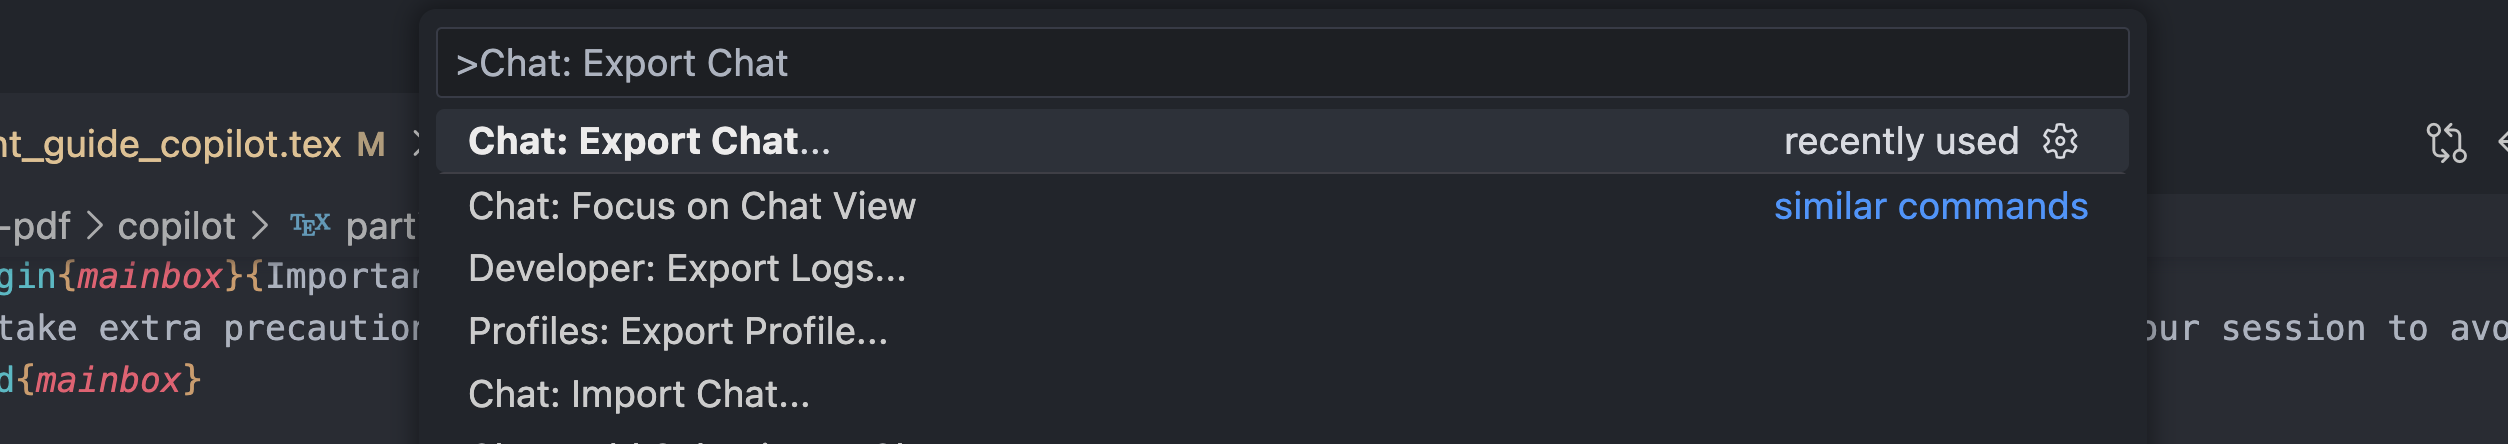
\includegraphics[width=1\textwidth]{assets/copilot/copilot-export-chat-command.png}
    \end{center}
    \item Name the exported \inlinecode{.json} file appropriately (e.g., use the agent name for APM conversations) and choose a location on your local machine to save.  \begin{center}
        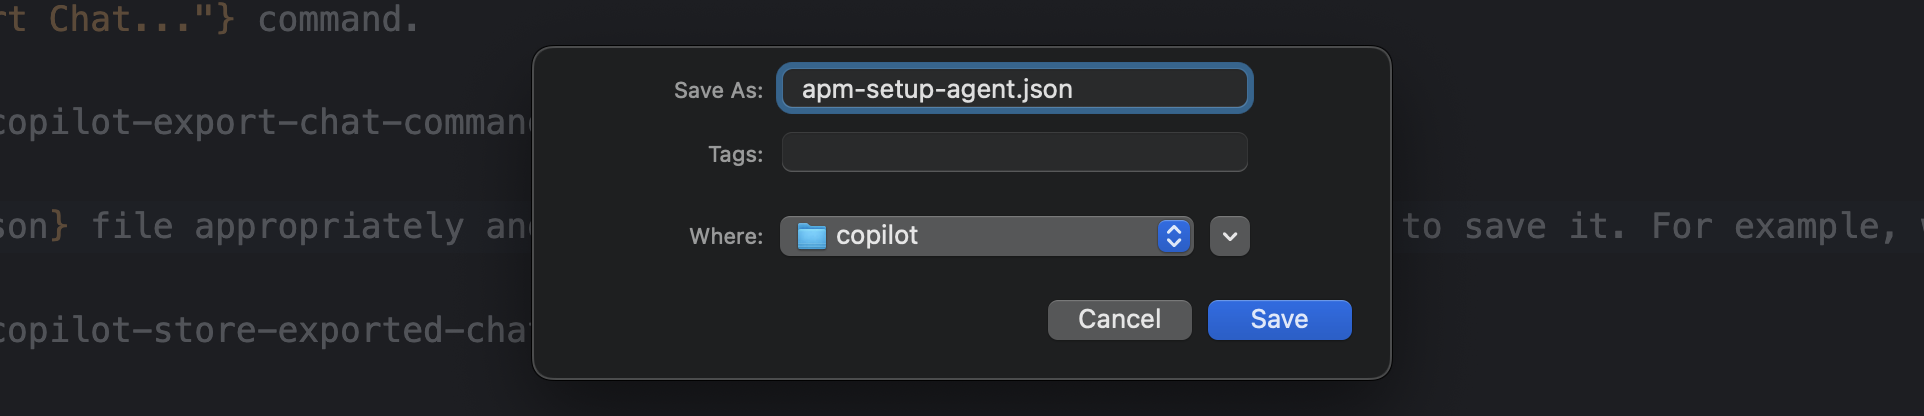
\includegraphics[width=1\textwidth]{assets/copilot/copilot-store-exported-chat.png}
    \end{center}
\end{itemize}
\noindent Repeat this process for all conversations used during the session. Once all conversations are exported, compress them into a single archive named \inlinecode{tool\_a\_chat\_conversations\_json.zip} for Tool A and \inlinecode{tool\_b\_chat\_conversations\_json.zip} for Tool B.
\begin{mainbox}{Important Chat Export Note}
To take extra precautions, consider exporting conversations \textbf{immediately after completion} your session to avoid accidental deletions or technical issues. For example, in APM the Setup Agent conversation can be exported right after the Setup Phase is complete.
\end{mainbox}

\newpage
% ============================================================================

\subsection{Retrieve AI Request Usage}

Copilot does not provide a detailed, time-stamped CSV of token usage, cost and other metrics per request. Instead, we will capture your total request usage through Copilot's Settings.

\begin{itemize}
    \item At the \textbf{start and end of your session}, open \href{https://github.com/settings/copilot/features}{GitHub's Copilot Settings}.
    \item In the \textbf{Usage} section, take a screenshot of the \textbf{Premium Requests percentage bar}. The difference between the start and end screenshots will be used to estimate your Copilot requests for the session.
    \begin{center}
        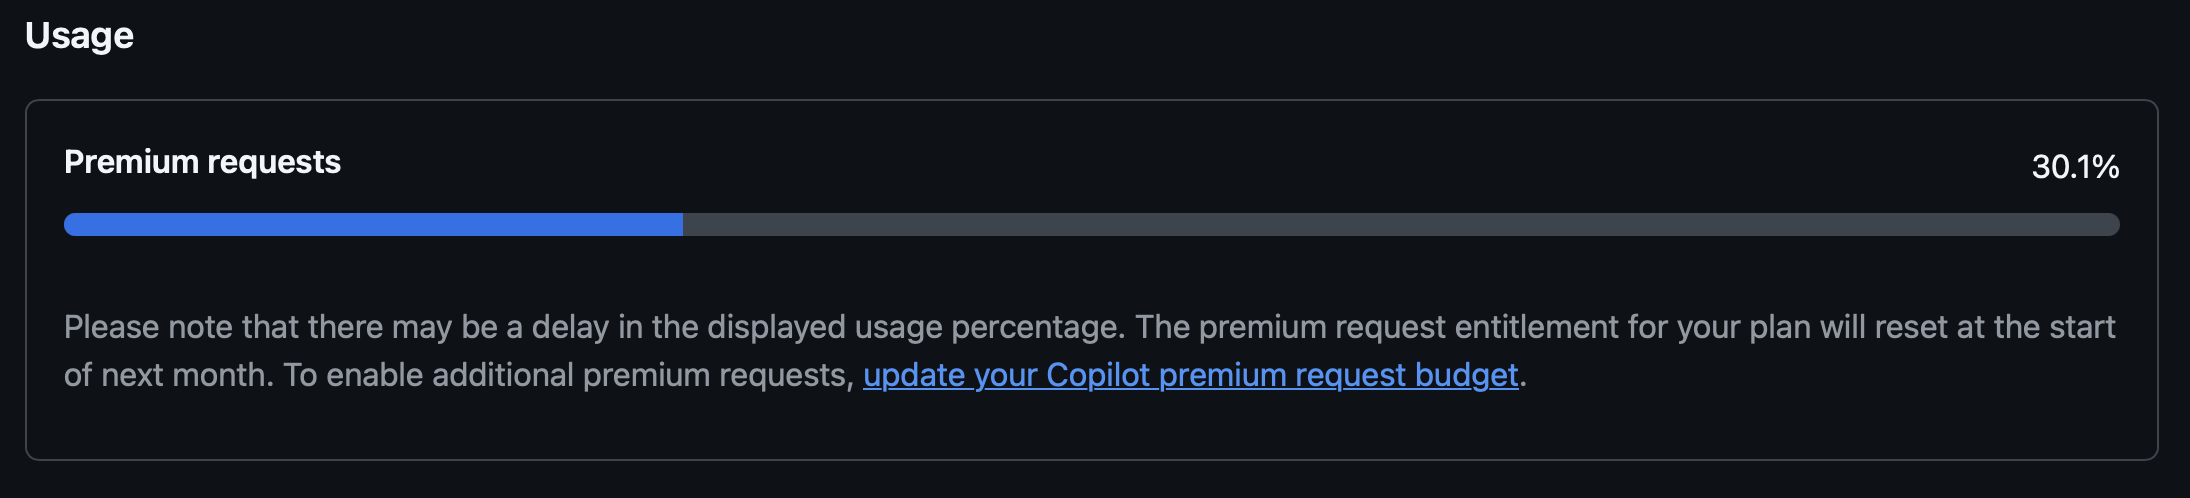
\includegraphics[width=1\textwidth]{assets/copilot/copilot-usage-screenshot.png}
    \end{center}
    \item Save the screenshots using proper naming: \inlinecode{tool\_a\_copilot\_requests\_start.png} and \inlinecode{tool\_a\_copilot\_requests\_end.png} for Tool A, and \inlinecode{tool\_b\_copilot\_requests\_start.png} and \inlinecode{tool\_b\_copilot\_requests\_end.png} for Tool B.
\end{itemize}

\begin{mainbox}{Important Note on Request Metrics}
We acknowledge this metric is less granular. The primary data for this study will come from the detailed \textbf{JSON chat exports}, which allow us to analyze the interaction patterns. The request count provides a secondary, high-level overview.
\end{mainbox}

\subsection{Package Logs for Submission}

Finally, compress the exported chat conversations and your request count screenshot into a single archive for submission. For example:
\begin{codebox}
zip -r tool_a_logs.zip tool_a_chat_conversations_json.zip tool_a_copilot_requests_start.png tool_a_copilot_requests_end.png
\end{codebox}
\subsection{Log Archives Summary}

After completing the above steps for both sessions, you will have two log archives: 
\begin{itemize}
    \item \inlinecode{tool\_a\_logs.zip} for Tool A
    \item \inlinecode{tool\_b\_logs.zip} for Tool B
\end{itemize}
These will be submitted along with your code patches in the final submission step.

\newpage
% ============================================================================

\section{Final Submission}

After completing both sessions, submit all your data to our \href{https://forms.gle/gzYNsSZwMbUDJRji6}{anonymous collection form}.

\subsection*{Submission Checklist}

Please be sure to upload the following files:

\begin{codebox}
    tool_a_solution.patch          # Code patch from Tool A session
    tool_b_solution.patch          # Code patch from Tool B session
    tool_a_logs.zip                # AI interaction logs from Tool A session
    tool_b_logs.zip                # AI interaction logs from Tool B session
\end{codebox}


\section{Contact \& Help}

This study is conducted for a Bachelor's thesis by Kostantinos Chaidemenos - \href{https://github.com/sdi2200262}{CobuterMan}.\newline\newline
If you encounter any technical issues or have questions about the study procedure, contact: 
\begin{codebox}
sdi2200262@di.uoa.gr        # Email
cobuter_man                 # Discord
\end{codebox}

\vspace{1cm}
\hrule height 0.3pt
\vspace{0.7cm}

\begin{center}
    \subsubsection*{\centering Thank you again for your time and contribution to this research.}
    
\includegraphics[width=0.3\textwidth]{assets/common/cobuter-man.png}
\end{center}

% ============================================================================

\end{document}